\section{Vector fields}
\begin{frame}{Vector fields}
\begin{columns}
\begin{column}{0.7\textwidth}
Let \( T:\mm_2\to\Kzt \) be an oriented tangent bundle on a 2-dim cellular type
\begin{itemize}
\item A \alert{vector field} is a term \alert{\( X:\pit{m:\mm_1}Tm \)}.
\item It's a \alert{nonvanishing} vector field on the 1-skeleton.
\item We model classical zeros by omitting the faces.
\end{itemize}
\end{column}
\begin{column}{0.3\textwidth}
\begin{tikzpicture}%
  [x={(-0.860769cm, -0.121512cm)},
  y={(0.508996cm, -0.205391cm)},
  z={(-0.000053cm, 0.971107cm)},
  scale=1,
  back/.style={loosely dotted, thin},
  edge/.style={black, thick},
  arrow/.style={black, very thick, solid, -{Stealth[scale=0.8]}},
  facet/.style={fill=blue!95!black,fill opacity=0.0},
  vertex/.style={inner sep=1pt,circle,draw=green!25!black,fill=black,thick}]
%% Drawing the vertices in the front
%%
\begin{scope}[nodes=vertex]
\node[label=above right:\( b \)] at (-1, 1, 0) (b)     {};
\node[label=below:\( y \)] at (0, 0, -1.4) (y)    {};
\node[label=above:\( w \)] at (0, 0, 1.4)  (w)   {};
\node[label=above left:\( g \)] at (1, -1, 0) (g)    {};
\node[label=above left:\( r \)] at (1, 1, 0)  (r)   {};
\node[label=above right:\( o \)] at (-1, -1, 0) (o)    {};
\end{scope}
%% Drawing edges in the back
%%
\draw[edge,back,arrow] (o) -- (b);
\draw[edge,back,arrow] (y) -- (o);
\draw[edge,back] (o) -- (w);
\draw[edge,back] (o) -- (g);
%% Drawing vertices in the back
%%
\node[vertex] at (o)     {};
%% Drawing the facets
%%
\fill[facet] (1, 1, 0) -- (0, 0, -1.4) -- (1, -1, 0) -- cycle {};
\fill[facet] (1, 1, 0) -- (0, 0, 1.4) -- (1, -1, 0) -- cycle {};
\fill[facet] (1, 1, 0) -- (-1, 1, 0) -- (0, 0, 1.4) -- cycle {};
\fill[facet] (1, 1, 0) -- (-1, 1, 0) -- (0, 0, -1.4) -- cycle {};
%% Drawing edges in the front
%%
\draw[edge,arrow] (b) -- (y);
\draw[edge] (b) -- (w);
\draw[edge] (b) -- (r);
\draw[edge] (y) -- (g);
\draw[edge] (y) -- (r);
\draw[edge,arrow] (g) -- (w);
\draw[edge,arrow] (w) -- (r);
\draw[edge,arrow] (r) -- (g);
\end{tikzpicture}

\end{column}
\end{columns}
\end{frame}

\begin{frame}{Pathovers}
\begin{columns}
\begin{column}{0.55\textwidth}
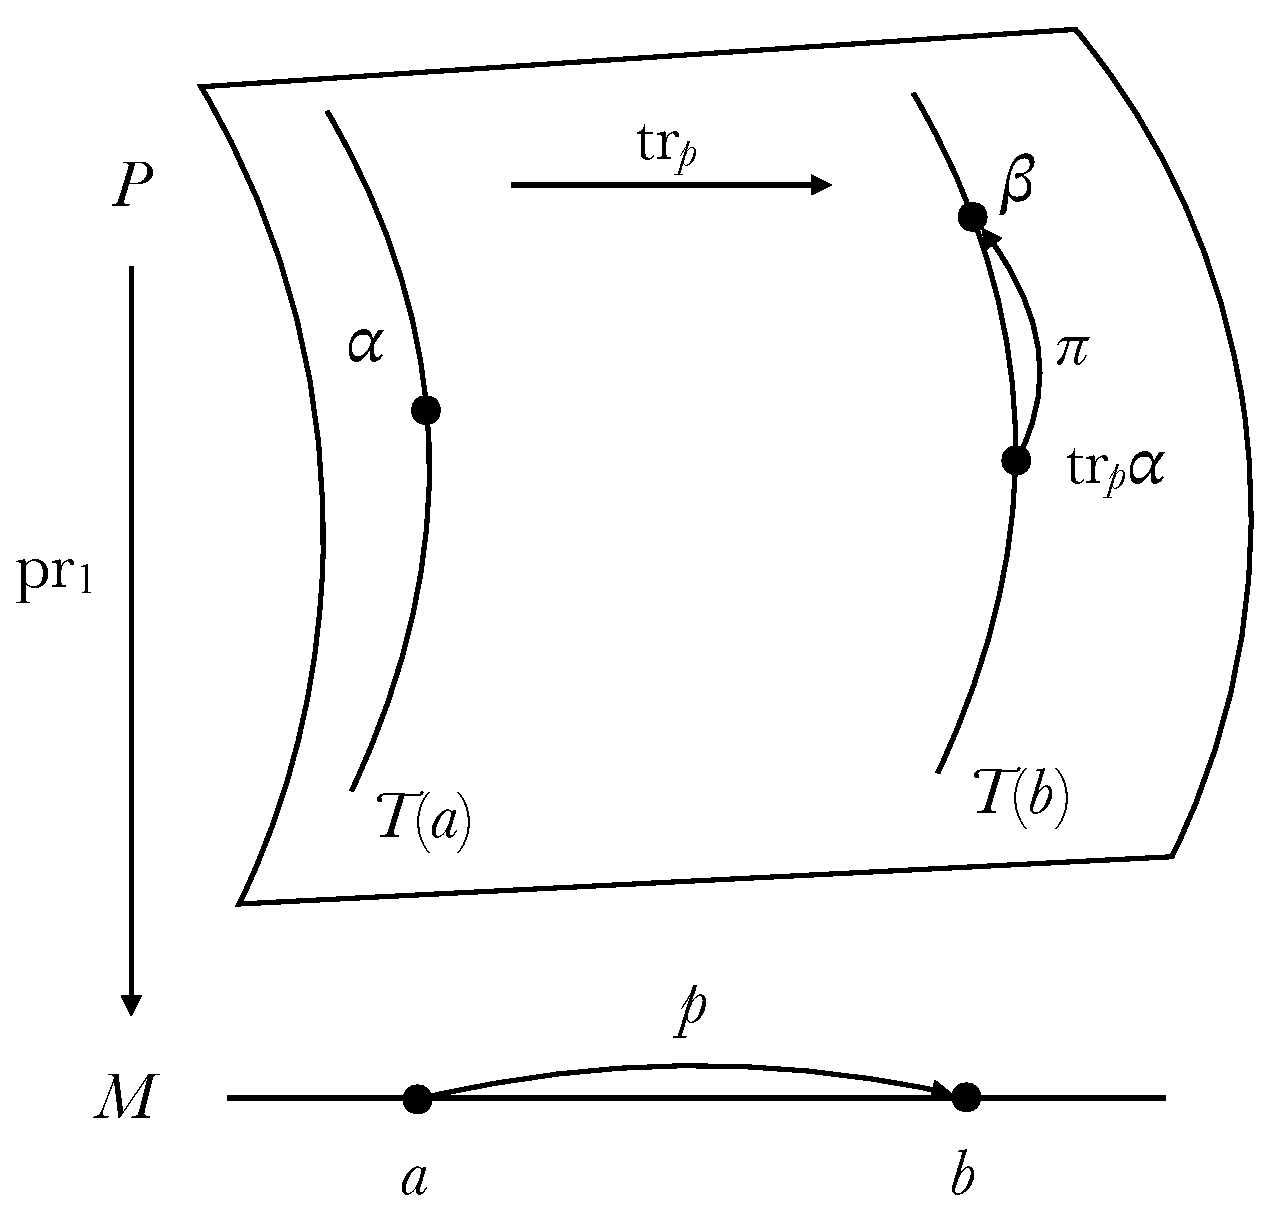
\includegraphics[width=30ex]{figs/pathovers.pdf}
\end{column}
\begin{column}{0.45\textwidth}
\begin{itemize}
\item Recall pathovers (dependent paths).
\item There is an asymmetry: we pick a fiber to display it.
\item Dependent functions map paths to pathovers (\( \apd \)).
\end{itemize}
\end{column}
\end{columns}
\end{frame}

\begin{frame}{Building up a triangle-over}
\begin{tikzcd}[ampersand replacement=\&, row sep=small]
  {T_1} \& {T_2} \& {T_3} \& {T_1} \\
  \&\&\& {T_{13}T_{32}T_{21}X_1} \\
  \&\& {T_{32}T_{21}X_1} \& {T_{13}T_{32}X_2} \\
  \& {T_{21}X_1} \& {T_{32}X_2} \& {T_{13}X_3} \\
  {X_1} \& {X_2} \& {X_3} \& {X_1}
  \arrow["{T_{21}}", from=1-1, to=1-2]
  \arrow["{T_{32}}", from=1-2, to=1-3]
  \arrow["{T_{13}}", from=1-3, to=1-4]
  \arrow["{\alert{T_{13}T_{32}X_{12}}:}", equals, from=3-4, to=2-4]
  \arrow["{\alert{X_{12}}:}"', equals, from=4-2, to=5-2]
  \arrow["{\alert{T_{32}X_{12}}:}", equals, from=4-3, to=3-3]
  \arrow["{\alert{T_{13}X_{23}}:}", equals, from=4-4, to=3-4]
  \arrow["{\alert{X_{23}}:}", equals, from=5-3, to=4-3]
  \arrow["{\alert{X_{31}}:}", equals, from=5-4, to=4-4]
\end{tikzcd}
\end{frame}

\begin{frame}
\begin{columns}
\begin{column}{0.65\textwidth}
\vspace{12pt}
\begingroup
\tikzset{every picture/.style={scale=0.85}}
\begin{tikzpicture}
  [arrow/.style={-{Stealth[scale=1.1]}}, vec/.style={ultra thick, color=black}, vectr/.style={thick, color=black}, vectrtr/.style={thick, dashed, color=black}, vectrtrtr/.style={thick, dotted, color=black}]
  \tikzset{oo/.style={circle, scale=0.6, fill=black}}
  \tikzset{ii/.style={circle, scale=0.3, fill=gray}}
  \setlength{\mylen}{3cm}
  \setlength{\mylin}{1.2cm}
    \node[oo, label=below right:\( v_1 \)] (V1) at (0, 0) {};
    \node[oo, label=below:\( v_3 \)] (V3) at (2*\mylen, 0) {};
    \node[oo, label=above:\( v_2 \)] (V2) at (\mylen, 1.732*\mylen) {};

    \draw[arrow] (V2) edge[very thick, color=teal, "\( e_{23} \)"] (V3);
    \draw[arrow] (V1) edge[very thick, color=magenta, "\( e_{12} \)"] (V2);
    \draw[arrow] (V3) edge[very thick, color=blue, "\( e_{31} \)"] (V1);
    
    \node [ii, above right=\mylin of V1] (V11) {};
    \node [ii, below right=\mylin of V1] (V14) {};
    \node [ii, below left=\mylin of  V1] (V13) {};
    \node [ii, above left= \mylin of V1] (V12) {};

    \node [left=1.3\mylin of  V1,  label=center:\( T_1 \)] {};
    \node [right=1.3\mylin of  V2,  label=center:\( T_2 \)] {};
    \node [right=1.3\mylin of  V3,  label=center:\( T_3 \)] {};

    \node [ii, above right=\mylin of V2] (V21) {};
    \node [ii, below right=\mylin of V2] (V24) {};
    \node [ii, below left=\mylin of  V2] (V23) {};
    \node [ii, above left= \mylin of V2] (V22) {};

    \node [ii, above right=\mylin of V3] (V31) {};
    \node [ii, below right=\mylin of V3] (V34) {};
    \node [ii, below left=\mylin of  V3] (V33) {};
    \node [ii, above left= \mylin of V3] (V32) {};

    \draw[dashed] (V11) -- (V12);
    \draw[dashed] (V12) -- (V13);
    \draw[dashed] (V13) -- (V14);
    \draw[dashed] (V14) -- (V11);

    \draw[dashed] (V21) -- (V22);
    \draw[dashed] (V22) -- (V23);
    \draw[dashed] (V23) -- (V24);
    \draw[dashed] (V24) -- (V21);
    
    \draw[dashed] (V31) -- (V32);
    \draw[dashed] (V32) -- (V33);
    \draw[dashed] (V33) -- (V34);
    \draw[dashed] (V34) -- (V31);
    
    \draw[arrow] (V1) edge[vec] (V11);
    \draw[arrow] (V2) edge[vectr] (V21);
    \draw[arrow] (V3) edge[vectrtr] (V34);
    \draw[arrow] (V1) edge[vectrtrtr] (V14);

    \draw[arrow] (V2) edge[vec] (V24);
    \draw[arrow] (V3) edge[vectr] (V33);
    \draw[arrow] (V1) edge[vectrtr] (V13);

    \draw[arrow] (V21) edge[thick, color=magenta] (V24);
    \draw[arrow] (V34) edge[thick, color=magenta] (V33);
    \draw[arrow] (V14) edge[thick, color=magenta] (V13);
    \draw[arrow] (V33) edge[thick, color=teal] (V32);
    \draw[arrow] (V13) edge[thick, color=teal] (V12);
    \draw[arrow] (V12) edge[thick, color=blue] (V11);

    \draw[arrow] (V3) edge[vec] (V32);
    \draw[arrow] (V1) edge[vectr] (V12);
\end{tikzpicture}

\endgroup
\end{column}
\begin{column}{0.35\textwidth}
\begin{itemize}
\item \( \partial F\defeq e_{12}\cdot e_{23}\cdot e_{31}.  \)
\item \( \tr \) thins out arrows.
\item \( X \) on a path is drawn in the path's color.
\item \( X(\partial F) \) traces 3 sides of a square.
\end{itemize}
\end{column}
\end{columns}
\end{frame}

\begin{frame}{Angle}
\begin{columns}
\begin{column}{0.3\textwidth}
\begin{tikzpicture}%
  [x={(-0.860769cm, -0.121512cm)},
  y={(0.508996cm, -0.205391cm)},
  z={(-0.000053cm, 0.971107cm)},
  scale=1,
  back/.style={loosely dotted, thin},
  edge/.style={black, thick},
  arrow/.style={black, very thick, solid, -{Stealth[scale=0.8]}},
  facet/.style={fill=blue!95!black,fill opacity=0.0},
  vertex/.style={inner sep=1pt,circle,draw=green!25!black,fill=black,thick}]
%% Drawing the vertices in the front
%%
\begin{scope}[nodes=vertex]
\node[label=above right:\( b \)] at (-1, 1, 0) (b)     {};
\node[label=below:\( y \)] at (0, 0, -1.4) (y)    {};
\node[label=above:\( w \)] at (0, 0, 1.4)  (w)   {};
\node[label=above left:\( g \)] at (1, -1, 0) (g)    {};
\node[label=above left:\( r \)] at (1, 1, 0)  (r)   {};
\node[label=above right:\( o \)] at (-1, -1, 0) (o)    {};
\end{scope}
%% Drawing edges in the back
%%
\draw[edge,back,arrow] (o) -- (b);
\draw[edge,back,arrow] (y) -- (o);
\draw[edge,back] (o) -- (w);
\draw[edge,back] (o) -- (g);
%% Drawing vertices in the back
%%
\node[vertex] at (o)     {};
%% Drawing the facets
%%
\fill[facet] (1, 1, 0) -- (0, 0, -1.4) -- (1, -1, 0) -- cycle {};
\fill[facet] (1, 1, 0) -- (0, 0, 1.4) -- (1, -1, 0) -- cycle {};
\fill[facet] (1, 1, 0) -- (-1, 1, 0) -- (0, 0, 1.4) -- cycle {};
\fill[facet] (1, 1, 0) -- (-1, 1, 0) -- (0, 0, -1.4) -- cycle {};
%% Drawing edges in the front
%%
\draw[edge,arrow] (b) -- (y);
\draw[edge] (b) -- (w);
\draw[edge] (b) -- (r);
\draw[edge] (y) -- (g);
\draw[edge] (y) -- (r);
\draw[edge,arrow] (g) -- (w);
\draw[edge,arrow] (w) -- (r);
\draw[edge,arrow] (r) -- (g);
\end{tikzpicture}

\end{column}
\begin{column}{0.7\textwidth}
\begin{itemize}
\item We want to extract from each \( X_{ij} \) just the \alert{angle}, a non-dependent quantity.
\item e.g. in this example: 3 copies of ``+1 notch'' and 3 of ``--1 notch.''
\item The total swirled angle is 0.
\end{itemize}
\end{column}
\end{columns}
\end{frame}

\begin{frame}{Angle}
\onslide<1->{Observation 1: Use the torsor structure. If we choose \( m:\mm \) then \( T_m=T_m \) acts on all fibers. We can define subtraction \( T_i\times T_i\to(T_m=T_m) \).}

\onslide<2->{Observation 2: Use the vector field. Given \( X_i:T_i \) we can form subtraction \( -X_i:T_i\to (T_m=T_m) \). \( X_{ij}-X_j:T_{ji}X_i-X_j=_{T_m=T_m}0 \).}

\onslide<3->{Observation 3: Use \( \ap \) of addition. We can add \( \alpha:a=_{\ccc(4)}0 \) and \( \beta:b=_{\ccc(4)}0 \) to form \( \alpha+\beta:(a+b)=_{\ccc(4)}0 \).}

\onslide<4->{Together these remove the dependency. We can compute \( \flat, I, X \) on each face independently and total them in \( T_m=T_m \).}
\end{frame}

\begin{frame}
\begin{lemma}
If \( G \) is a higher group with multiplication \( \mu:G\times G\to G \) and proof of commutativity \( \mathsf{is\underscore comm}:\pit{a,b:G}\mu(a, b)=\mu(b, a) \) then \( \mu \) induces a function \( \mu_=:(x=_G y)\times (x'=_G y')\to (\mu(x, x')=_G\mu(y,y')) \).
\end{lemma}
\begin{proof}
If \( p:x=_G y \) and \( p':x'=_G y' \), then we can define \( \mu_=(p, p') \) by concatenating the three paths 
\begin{align*} 
\mu(x',p)&:\mu(x', x)=_G\mu(x', y)\\
\mathsf{is\underscore comm}(x',y)&:\mu(x',y)=_G\mu(y,x')\\
\mu(y, p')&:\mu(y, x')=_G\mu(y, y').\qedhere
\end{align*}
\end{proof}
\end{frame}

\begin{frame}
\[\begin{aligned}
\tr_F&\defeq \tr(\partial F)&&:T_1=_{\Kzt}T_1&&\text{\alert{holonomy}}\\
\flat_F&\defeq \flat(\partial F)&&:\id=_{T_1=T_1}\tr_F&&\text{\alert{flatness}}\\
X_F&\defeq X(\partial F)&&:\tr_F(X_1)=_{T_1}X_1&&\text{\alert{swirling}}\\
\end{aligned}\]
\onslide<2->{
\begin{columns}[c]
\begin{column}{0.7\textwidth}
\begin{mydef}
The \defemph{index of the vector field \( X \) on the face \( F \)} is the integer \( I^X_F\defeq\loopy(\flat_F(X_1)\cdot X_F):\loopy(X_1=_{T_1}X_1) \).
\end{mydef}
\end{column}
\begin{column}{0.3\textwidth}
\begin{tikzpicture}
  [arrow/.style={-{Stealth[scale=1.1]}}, .style={scale=0.7}]
  \tikzset{oo/.style={circle, scale=0.6, fill=black}}
  \tikzset{ii/.style={circle, scale=0.3, fill=gray}}
  \setlength{\mylen}{2cm}
  \setlength{\mylin}{1cm}
  \node[label=center:\( Tv_1 \)] (V1) at (0, 0) {};
  \node [ii, above right=\mylin of V1,  label=right:\( v_{11} \)] (V11) {};
  \node [ii, below right=\mylin of V1,  label=right:\( v_{12} \)] (V12) {};
  \node [ii, below left=\mylin of  V1,  label=left:\( v_{13} \)] (V13) {};
  \node [ii, above left= \mylin of V1,  label=left: \( v_{14} \)] (V14) {};

  \draw[dashed] (V11) edge[ultra thick, solid, arrow, swap, "\( \flat_F(X_1) \)"] (V14);
  \draw[arrow] (V14) edge[thick, swap, color=magenta, "\( X_{12} \)"] (V13);
  \draw[arrow] (V13) edge[thick, swap, color=teal, "\( X_{23} \)"] (V12);
  \draw[arrow] (V12) edge[thick, swap, color=blue, "\( X_{31} \)"] (V11);
\end{tikzpicture}
\end{column}
\end{columns}}
\end{frame}

